\documentclass{beamer}

\usepackage{verbatim}

\usetheme{CambridgeUS}

\usecolortheme{dolphin}

%\setbeamertemplate{footline}[page number]

\setbeamertemplate{navigation symbols}{}

\title{Git}
\author{Java Cursisten}
\institute{INTEC Brussel}
\date{\today}

\begin{document}


\begin{frame}

\titlepage

\end{frame}


\begin{frame}

\frametitle{Overzicht}
{\LARGE \tableofcontents}

\end{frame}


\section{Wat is version control?}


\begin{frame}

\frametitle{Dagelijkse taken van een programmeur}

\begin{itemize}
\item {\LARGE Create (new Class)}
\item {\LARGE Save}
\item {\LARGE Edit}
\item {\LARGE Save... again...}
\end{itemize} 

\end{frame}


\begin{frame}

\frametitle{Save... again... and again...}

{\LARGE Hier komt version control helpen}\\~\\

\begin{itemize}
\item {\LARGE Wie} 
\item {\LARGE Wanneer aangepast}
\item {\LARGE Waarom aangepast}
\item {\LARGE Wat aangepast}\\~\\
\end{itemize}

{\LARGE Wordt bijgehouden en kan ten alle tijden bekeken worden}

\end{frame}


\begin{frame}

{\LARGE Voor \'e\'en bestand voor \'e\'en persoon nog relatief triviaal\\~\\

Bij samenwerking komt version control past echt helpen.\\~\\

Als meerdere gebruikers onafhankelijk van elkaar verschillende aanpassingen
hebben doorgevoerd moeten deze samenkomen... a merge.\\~\\}

\end{frame}


\begin{frame}

\frametitle{Grafische voorstelling}

\begin{figure}

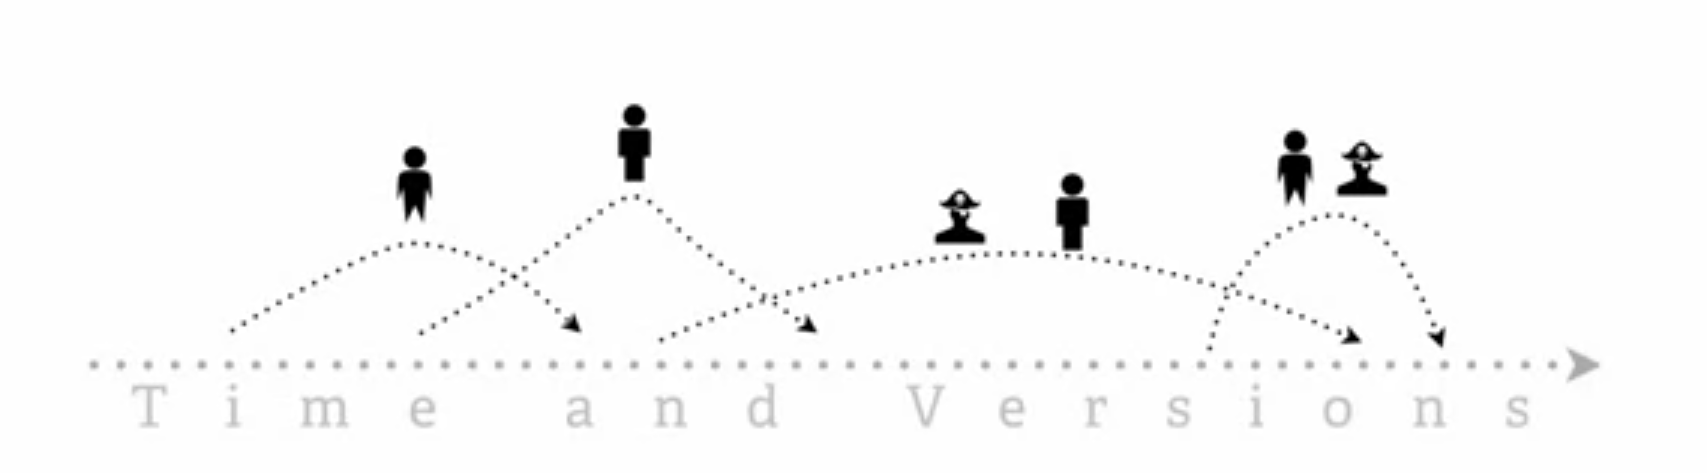
\includegraphics[width=350pt]{Grafiek.png}

\end{figure}

\end{frame}


\section{Wat is Git?}


\begin{frame}

\frametitle{Wat is Git}

\begin{itemize}
\item {\LARGE snelle en moderne implementatie van version control (2005)}
\item {\LARGE Git geeft u een geschiedenis van veranderingen van al de bestanden}
\item {\LARGE Git maakt dit mogelijk met veranderingen door verschillende personen (100+)}
\item {\LARGE Git kan gebruikt worden door elke 'knowledge worker' (progammeur,  architect, fotograaf, schrijver, ...)}
\end{itemize}

\end{frame}


\begin{frame}

\frametitle{Wat is Git?}

{\LARGE Git is een {\huge \textbf{gedistribueerd}} systeem.\\~\\

Iedere gebruiker heeft zijn eigen kopie van het werk waar hij lokaal (offline) mee kan doen wat hij wil.\\~\\}

\end{frame}


\begin{frame}

\frametitle{Git concepten}

{\Large \begin{itemize}
\item repository : een locatie van de bestanden en bijhorend 'dagboek'
\item clone : een remote repository van een andere eigenaar kopi\"eren naar een nieuwe local repository (veelal eerste stap)
\item pull : om uw local repository up to date te brengen met remote repository
\item push : om uw remote repository up to date te brengen met local repository
\item pull request : vragen of de eigenaar van een repository uw veranderingen pulled (fetch \& merge)
\end{itemize}}

\end{frame}


\begin{frame}

\frametitle{Meer informatie}

{\huge \href{http://git-scm.com/book/nl}{Link : Git Pro (nederlands)}}

\end{frame}


\section{Wat is GitHub?}


\begin{frame}

\frametitle{GitHub}

{\Large GitHub is een hosting service voor Git repositories.\\~\\

Maakt samenwerking makkelijker op te zetten omdat er niemand
zelf een server moet opzetten.\\~\\

\href{https://github.com/}{Link naar GitHub site}\\~\\

Wij gaan github:windows gebruiken om met Git en GitHub te werken omdat dit
alles veel gemakkelijker maakt.\\~\\

\href{http://windows.github.com/}{Link naar github:windows} }

\end{frame}


\begin{frame}

\frametitle{Hackfest(je)}

{\Large Doel :

\begin{itemize}
\item GitHub voor windows installeren en opzetten
\item eigen repository opzetten en pushen naar GitHub\\ (iets wat je wilt 'version controllen')
\item pullen van {\footnotesize \url{https://github.com/VanbockryckInstructeur/JavaLaTeXBestanden}}
\item JavaLaTeXBestanden aanpassen en pull request doen
\item Mergen
\end{itemize}}

\end{frame}


\end{document}